%!TEX TS-program = pdflatex
%!TEX TS-options = -shell-escape
\newcommand{\setfontsize}{11pt}
\documentclass[%
	paper=a4,
	fontsize=\setfontsize,
	ngerman
	]{scrartcl}

% Basics für Codierung und Sprache
% ===========================================================
	\usepackage{scrtime}
	\usepackage{etex}
	\usepackage{shellesc}
	\usepackage[final]{graphicx}
	\usepackage[utf8]{inputenc}
	\usepackage{babel}
	\usepackage[german=quotes]{csquotes}
% ===========================================================

% Fonts und Typographie
% ===========================================================
	\usepackage{sourcecodepro}
	\usepackage[default]{sourcesanspro}
	\usepackage{nimbusmononarrow}
	
	\usepackage[babel=true,final,tracking=smallcaps]{microtype}
	\DisableLigatures{encoding = T1, family = tt* } % keine Ligaturen für Monospace-Fonts
	\usepackage{ellipsis}
% ===========================================================

% Farben
% ===========================================================
	\usepackage[usenames,x11names,final]{xcolor}
	\definecolor{fbblau}{HTML}{3078AB}
	\definecolor{mediumgray}{gray}{.65}
	\definecolor{blackberry}{rgb}{0.53, 0.0, 0.25}
% ===========================================================

% Mathe-Pakete und -Einstellungen
% ===========================================================
	\usepackage{mathtools}
	\usepackage{amssymb}
	\usepackage[bigdelims]{newtxmath}		% moderne Mathe-Font
	\allowdisplaybreaks						% seitenübergreifende Rechnungen
	\input{../MathCmds.tex}
	\usepackage{bm}
	\usepackage{wasysym}
% ===========================================================

% TikZ
% ===========================================================
	\usepackage{tikz}
	\usepackage{tikz-cd}					% kommutative Diagramme
	\usetikzlibrary{arrows.meta}			% mehr Pfeile!
	\usetikzlibrary{shadows}
	\usetikzlibrary{calc}
	\tikzset{>=Latex}						% Standard-Pfeilspitze
% ===========================================================

% Seitenlayout, Kopf-/Fußzeile
% ===========================================================
	\usepackage{scrpage2}
	\pagestyle{scrheadings}
	\usepackage[top=3cm, bottom=3cm, left=2.5cm, right=2cm]{geometry}
	\clearscrheadfoot 
	\setheadsepline{0.4pt} 					% Linie in Kopfzeile
	\setfootsepline{0.4pt}
	\automark[section]{section}				% Abschnittstitel in Kopfzeile
	\setkomafont{pagehead}{\bfseries}
	\setkomafont{pagefoot}{\normalfont\footnotesize}
	\cfoot{\thepage}
	\raggedbottom
	\usepackage{setspace}					
	\onehalfspacing							% Zeilenabstand 1.5-fach
	\setlength{\parindent}{0pt}
	\setlength{\parskip}{0.5\baselineskip}
	\usepackage[all]{nowidow}
% ===========================================================

% Hyperref
% ===========================================================
	\usepackage[%
		hidelinks,
		pdfpagelabels,
		bookmarksopen=true,
		bookmarksnumbered=true,
		linkcolor=black,
		urlcolor=SkyBlue2,
		plainpages=false,
		pagebackref,
		citecolor=black,
		hypertexnames=true,
		pdfauthor={Phil Steinhorst},
		pdfborderstyle={/S/U},
		linkbordercolor=SkyBlue2,
		colorlinks=false,
		backref=false]{hyperref}
	\hypersetup{final}
% ===========================================================

% Listen und Tabellen
% ===========================================================
	\usepackage{multicol}
	\usepackage[shortlabels]{enumitem}
	\setlist{itemsep=0pt}
	\setlist[enumerate]{font=\sffamily\bfseries}
	\setlist[itemize]{label=$\triangleright$}
	\usepackage{tabularx}
% ===========================================================

% Zu Testzwecken
% ===========================================================
	\usepackage{lipsum}
% ===========================================================

% Rechnerstrukturenquatsch
% ===========================================================
	\usepackage{karnaughmap}
% ===========================================================

% ntheorem
% ===========================================================
	\usepackage[amsmath]{ntheorem}
	
	\theoremstyle{default}
	\theoremseparator{.}
	\theorembodyfont{\normalfont}
	\theorempreskip{2em}
	\theorempostskip{2em}
	\newtheorem{aufg}{Aufgabe}

% minted
% ===========================================================
\usepackage{minted}
\setminted{%
	style=bw,
	fontsize=\normalsize,
	breaklines,
	breakanywhere=false,
	breakbytoken=false,
	breakbytokenanywhere=false,
	breakafter={.,},
	autogobble,
	numbersep=3mm,
	tabsize=4,
	frame=lines
}
\setmintedinline{%
	style=bw,
	fontsize=\normalsize,
	numbers=none,
	numbersep=12pt,
	tabsize=4,
	%bgcolor=gray!15,
}

\usepackage[tikz]{mdframed}
\newcommand{\code}[1]{\texttt{#1}}
\lohead{C++-Übungsaufgaben (6)}
\rohead{25.02.2019}
\rofoot{\jobname.tex}
\lofoot{}
\begin{document}

Eine \textbf{Warteschlange} (engl. \textit{queue}) ist eine Datenstruktur, die aus einzelnen Knoten (engl. \textit{node}) besteht.
Jeder Knoten besitzt einen Wert eines fest gewählten Datentypen und einen Verweis auf den nächsten Knoten in der Warteschlange.
Die Besonderheit einer Warteschlange ist, dass ausschließlich auf den vordersten Knoten zugegriffen werden kann.
Neue Knoten werden stets hinter den letzten Knoten der Schlage angehängt. 

\begin{center}
	\begin{tikzpicture}[scale=0.8,every node/.style={scale=0.8}]
		%\draw[gray] (0,2) grid (14,-3);
		\draw [very thick] (0,0) rectangle (2.5,2);
		\draw (1.25,1.5) node{\textbf{Queue}};
		\draw (0,0) node[anchor=south west,align = left]{length = 4 \\ first = };
		
		\draw [very thick] (3,-0.5) rectangle (5,-2.5);
		\draw (4,-1) node[font=\small]{\textbf{QueueNode}};
		\draw (3,-2.5) node[font=\small,anchor=south west,align = left]{data = 42 \\ next = };
		
		\draw [very thick] (6,-0.5) rectangle (8,-2.5);
		\draw (7,-1) node[font=\small]{\textbf{QueueNode}};
		\draw (6,-2.5) node[font=\small,anchor=south west,align = left]{data = 13 \\ next = };
		
		\draw [very thick] (9,-0.5) rectangle (11,-2.5);
		\draw (10,-1) node[font=\small]{\textbf{QueueNode}};
		\draw (9,-2.5) node[font=\small,anchor=south west,align = left]{data = 37 \\ next = };
		
		\draw [very thick] (12,-0.5) rectangle (14,-2.5);
		\draw (13,-1) node[font=\small]{\textbf{QueueNode}};
		\draw (12,-2.5) node[font=\small,anchor=south west,align = left]{data = 249 \\ next = $\emptyset$ };
		
		\draw[->,thick] (1.1,0.3) -- (4,0.3) -- (4,-0.5);
		\draw[->,thick] (4.1,-2.2) -- (5.2,-2.2) -- (5.2,-1) -- (6,-1);
		\draw[->,thick] (7.1,-2.2) -- (8.2,-2.2) -- (8.2,-1) -- (9,-1);
		\draw[->,thick] (10.1,-2.2) -- (11.2,-2.2) -- (11.2,-1) -- (12,-1);
	\end{tikzpicture}
\end{center}


In dieser Aufgabe soll eine Warteschlange für beliebige Datentypen implementiert werden.
Dafür sind folgende Klassendiagramme gegeben:

\begin{center}
	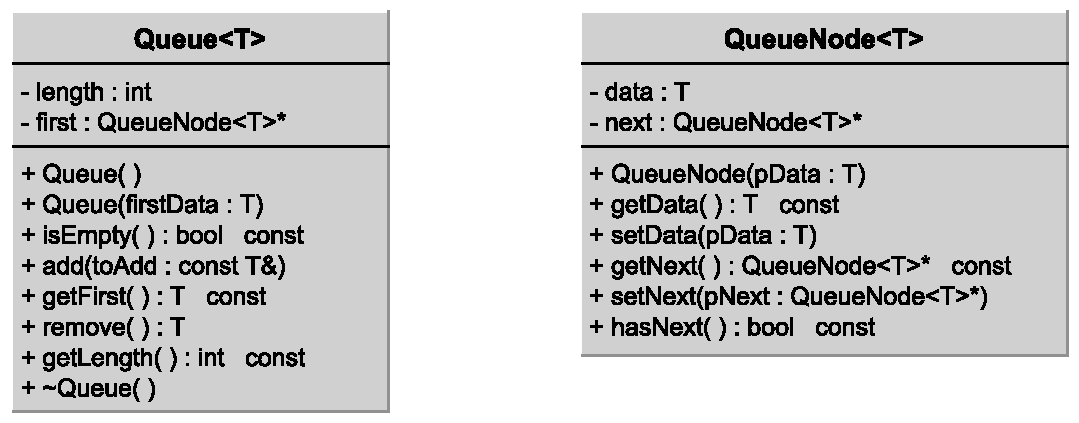
\includegraphics[keepaspectratio,scale=0.6]{Queue-uml.pdf}
\end{center}

\begin{enumerate}
	\item Implementieren Sie das Klassendiagramm der generischen Klasse \code{QueueNode}, mit welcher die Knoten einer Warteschlange realisiert werden.
	\begin{itemize}
		\item Der Konstruktor zur Erzeugung eines neuen Knotens erhält den im Knoten zu speichernden Wert. Der Nachfolger eines neuen Knotens ist zunächst nicht definiert.
		\item Die Methode \code{hasNext} gibt \code{true} zurück, falls ein Knoten einen Nachfolger besitzt.
	\end{itemize}
	\item Implementieren Sie das Klassendiagramm der generischen Klasse \code{Queue}, indem Sie Ihre Implementation von \code{QueueNode} nutzen.
	\begin{itemize}
		\item Der erste Konstruktor erzeugt eine neue Warteschlange ohne Elemente.
		\item Der zweite Konstruktor setzt zusätzlich den übergebenen Wert als ersten Wert der Schlange.
		\item Die Methode \code{add} fügt den übergebenen Wert ans Ende der Schlange ein.
		\item Die Methode \code{getFirst} liefert den ersten Wert der Schlange.
		\item Die Methode \code{remove} entfernt zusätzlich den ersten Wert aus der Schlage.
	\end{itemize}
	\item Erstellen Sie eine \code{main}-Methode, in der Sie eine Warteschlange für \code{int}-Werte erstellen.
	Fügen Sie ein paar Werte in die Warteschlange ein.
	Geben Sie anschließend alle Werte in der Warteschlange auf der Konsole aus.
\end{enumerate}
\end{document}